% Generated by scripts/generate_empirical_kernel_component_figures.py; do not edit manually.
% calibration root: outputs/depth_kernel_calibration/20260717_145624_rank_pooled_top10_h10
% source RISANAMENTO: outputs/depth_kernel_calibration/20260717_145624_rank_pooled_top10_h10/RISANAMENTO_top10_h10/empirical_depth_kernel.csv sha256=6ecb2071cf524f6090dff6596dc64248cbf59af2c55cf0d33e0649fcc52abe45
% source NEXI: outputs/depth_kernel_calibration/20260717_145624_rank_pooled_top10_h10/NEXI_top10_h10/empirical_depth_kernel.csv sha256=deaeb5a1c7a301d48c51347fbc4bdc2dc389281302aeb41192c20190920335f5
% source FERRARI: outputs/depth_kernel_calibration/20260717_145624_rank_pooled_top10_h10/FERRARI_top10_h10/empirical_depth_kernel.csv sha256=d5fdc562b059874471a511f2990341ceed08f434ddefb8b3cf31589979a67540

% data column: visibility_component
\begin{figure}[!ht]
\centering
\resizebox{\textwidth}{!}{%
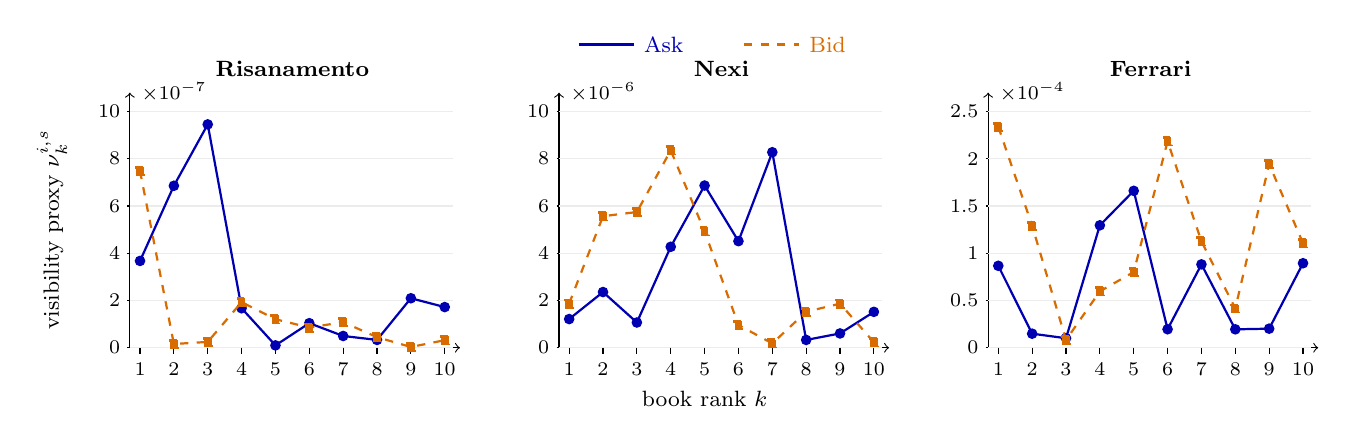
\begin{tikzpicture}
\begin{scope}[xshift=0.00cm]
\begin{scope}[x=0.43cm,y=0.30000000cm]
  \draw[->] (0.7,0) -- (10.45,0);
  \draw[->] (0.7,0) -- (0.7,10.8);
  \draw[gray!15] (0.7,0) -- (10.25,0);
  \draw (0.63,0) -- (0.7,0) node[left,font=\scriptsize] {0};
  \draw[gray!15] (0.7,2) -- (10.25,2);
  \draw (0.63,2) -- (0.7,2) node[left,font=\scriptsize] {2};
  \draw[gray!15] (0.7,4) -- (10.25,4);
  \draw (0.63,4) -- (0.7,4) node[left,font=\scriptsize] {4};
  \draw[gray!15] (0.7,6) -- (10.25,6);
  \draw (0.63,6) -- (0.7,6) node[left,font=\scriptsize] {6};
  \draw[gray!15] (0.7,8) -- (10.25,8);
  \draw (0.63,8) -- (0.7,8) node[left,font=\scriptsize] {8};
  \draw[gray!15] (0.7,10) -- (10.25,10);
  \draw (0.63,10) -- (0.7,10) node[left,font=\scriptsize] {10};
  \draw (1,0) -- (1,-0.025 * 10) node[below,font=\scriptsize] {1};
  \draw (2,0) -- (2,-0.025 * 10) node[below,font=\scriptsize] {2};
  \draw (3,0) -- (3,-0.025 * 10) node[below,font=\scriptsize] {3};
  \draw (4,0) -- (4,-0.025 * 10) node[below,font=\scriptsize] {4};
  \draw (5,0) -- (5,-0.025 * 10) node[below,font=\scriptsize] {5};
  \draw (6,0) -- (6,-0.025 * 10) node[below,font=\scriptsize] {6};
  \draw (7,0) -- (7,-0.025 * 10) node[below,font=\scriptsize] {7};
  \draw (8,0) -- (8,-0.025 * 10) node[below,font=\scriptsize] {8};
  \draw (9,0) -- (9,-0.025 * 10) node[below,font=\scriptsize] {9};
  \draw (10,0) -- (10,-0.025 * 10) node[below,font=\scriptsize] {10};
  \node[anchor=south west,font=\scriptsize] at (0.75,10) {$\times 10^{-7}$};
  \node[rotate=90,font=\footnotesize] at (-1.6,5) {visibility proxy $\nu_k^{i,s}$};
  \node[font=\footnotesize\bfseries] at (5.5,11.8) {Risanamento};
  \draw[blue!70!black, thick, mark=*, mark size=1.5pt] plot coordinates {(1,3.675229767983178) (2,6.855802152861837) (3,9.454395390358135) (4,1.6711452429542564) (5,0.09967103872544607) (6,1.03986078936913) (7,0.49722130939049286) (8,0.331027311346062) (9,2.094561089973038) (10,1.7209334991488594)};
  % RISANAMENTO ask visibility_component raw: 1:3.6752297679831775e-07, 2:6.855802152861836e-07, 3:9.4543953903581345e-07, 4:1.6711452429542563e-07, 5:9.9671038725446058e-09, 6:1.03986078936913e-07, 7:4.9722130939049281e-08, 8:3.31027311346062e-08, 9:2.0945610899730381e-07, 10:1.7209334991488592e-07
  \draw[orange!85!black, thick, dashed, mark=square*, mark size=1.4pt] plot coordinates {(1,7.4850054933810215) (2,0.15725764971410325) (3,0.24659322933232064) (4,1.930205433978854) (5,1.2069432758813796) (6,0.8540517059063696) (7,1.0836250920231838) (8,0.4466903180509029) (9,0.031098089940439774) (10,0.31967530278917544)};
  % RISANAMENTO bid visibility_component raw: 1:7.4850054933810209e-07, 2:1.5725764971410324e-08, 3:2.4659322933232062e-08, 4:1.9302054339788539e-07, 5:1.2069432758813797e-07, 6:8.5405170590636958e-08, 7:1.0836250920231838e-07, 8:4.4669031805090292e-08, 9:3.1098089940439771e-09, 10:3.1967530278917541e-08
\end{scope}
\end{scope}
\begin{scope}[xshift=5.45cm]
\begin{scope}[x=0.43cm,y=0.30000000cm]
  \draw[->] (0.7,0) -- (10.45,0);
  \draw[->] (0.7,0) -- (0.7,10.8);
  \draw[gray!15] (0.7,0) -- (10.25,0);
  \draw (0.63,0) -- (0.7,0) node[left,font=\scriptsize] {0};
  \draw[gray!15] (0.7,2) -- (10.25,2);
  \draw (0.63,2) -- (0.7,2) node[left,font=\scriptsize] {2};
  \draw[gray!15] (0.7,4) -- (10.25,4);
  \draw (0.63,4) -- (0.7,4) node[left,font=\scriptsize] {4};
  \draw[gray!15] (0.7,6) -- (10.25,6);
  \draw (0.63,6) -- (0.7,6) node[left,font=\scriptsize] {6};
  \draw[gray!15] (0.7,8) -- (10.25,8);
  \draw (0.63,8) -- (0.7,8) node[left,font=\scriptsize] {8};
  \draw[gray!15] (0.7,10) -- (10.25,10);
  \draw (0.63,10) -- (0.7,10) node[left,font=\scriptsize] {10};
  \draw (1,0) -- (1,-0.025 * 10) node[below,font=\scriptsize] {1};
  \draw (2,0) -- (2,-0.025 * 10) node[below,font=\scriptsize] {2};
  \draw (3,0) -- (3,-0.025 * 10) node[below,font=\scriptsize] {3};
  \draw (4,0) -- (4,-0.025 * 10) node[below,font=\scriptsize] {4};
  \draw (5,0) -- (5,-0.025 * 10) node[below,font=\scriptsize] {5};
  \draw (6,0) -- (6,-0.025 * 10) node[below,font=\scriptsize] {6};
  \draw (7,0) -- (7,-0.025 * 10) node[below,font=\scriptsize] {7};
  \draw (8,0) -- (8,-0.025 * 10) node[below,font=\scriptsize] {8};
  \draw (9,0) -- (9,-0.025 * 10) node[below,font=\scriptsize] {9};
  \draw (10,0) -- (10,-0.025 * 10) node[below,font=\scriptsize] {10};
  \node[anchor=south west,font=\scriptsize] at (0.75,10) {$\times 10^{-6}$};
  \node[font=\footnotesize\bfseries] at (5.5,11.8) {Nexi};
  \draw[blue!70!black, thick, mark=*, mark size=1.5pt] plot coordinates {(1,1.2138032154980023) (2,2.357195510456608) (3,1.0685006264223715) (4,4.273217243409157) (5,6.866026041374058) (6,4.512030446576142) (7,8.275878917434618) (8,0.32997233355025435) (9,0.6049414509297961) (10,1.5188249155682871)};
  % NEXI ask visibility_component raw: 1:1.2138032154980023e-06, 2:2.357195510456608e-06, 3:1.0685006264223715e-06, 4:4.2732172434091567e-06, 5:6.8660260413740573e-06, 6:4.5120304465761415e-06, 7:8.2758789174346172e-06, 8:3.2997233355025434e-07, 9:6.0494145092979615e-07, 10:1.5188249155682871e-06
  \draw[orange!85!black, thick, dashed, mark=square*, mark size=1.4pt] plot coordinates {(1,1.8674773855957816) (2,5.568884213770531) (3,5.7442838166896815) (4,8.353844420062963) (5,4.925771459538285) (6,0.9619962140487628) (7,0.1805094913160257) (8,1.5237267589959187) (9,1.8662709068477343) (10,0.2317283350241909)};
  % NEXI bid visibility_component raw: 1:1.8674773855957815e-06, 2:5.5688842137705302e-06, 3:5.7442838166896813e-06, 4:8.3538444200629627e-06, 5:4.9257714595382846e-06, 6:9.6199621404876272e-07, 7:1.8050949131602569e-07, 8:1.5237267589959187e-06, 9:1.8662709068477342e-06, 10:2.3172833502419091e-07
\end{scope}
\end{scope}
\begin{scope}[xshift=10.90cm]
\begin{scope}[x=0.43cm,y=1.20000000cm]
  \draw[->] (0.7,0) -- (10.45,0);
  \draw[->] (0.7,0) -- (0.7,2.7);
  \draw[gray!15] (0.7,0) -- (10.25,0);
  \draw (0.63,0) -- (0.7,0) node[left,font=\scriptsize] {0};
  \draw[gray!15] (0.7,0.5) -- (10.25,0.5);
  \draw (0.63,0.5) -- (0.7,0.5) node[left,font=\scriptsize] {0.5};
  \draw[gray!15] (0.7,1) -- (10.25,1);
  \draw (0.63,1) -- (0.7,1) node[left,font=\scriptsize] {1};
  \draw[gray!15] (0.7,1.5) -- (10.25,1.5);
  \draw (0.63,1.5) -- (0.7,1.5) node[left,font=\scriptsize] {1.5};
  \draw[gray!15] (0.7,2) -- (10.25,2);
  \draw (0.63,2) -- (0.7,2) node[left,font=\scriptsize] {2};
  \draw[gray!15] (0.7,2.5) -- (10.25,2.5);
  \draw (0.63,2.5) -- (0.7,2.5) node[left,font=\scriptsize] {2.5};
  \draw (1,0) -- (1,-0.025 * 2.5) node[below,font=\scriptsize] {1};
  \draw (2,0) -- (2,-0.025 * 2.5) node[below,font=\scriptsize] {2};
  \draw (3,0) -- (3,-0.025 * 2.5) node[below,font=\scriptsize] {3};
  \draw (4,0) -- (4,-0.025 * 2.5) node[below,font=\scriptsize] {4};
  \draw (5,0) -- (5,-0.025 * 2.5) node[below,font=\scriptsize] {5};
  \draw (6,0) -- (6,-0.025 * 2.5) node[below,font=\scriptsize] {6};
  \draw (7,0) -- (7,-0.025 * 2.5) node[below,font=\scriptsize] {7};
  \draw (8,0) -- (8,-0.025 * 2.5) node[below,font=\scriptsize] {8};
  \draw (9,0) -- (9,-0.025 * 2.5) node[below,font=\scriptsize] {9};
  \draw (10,0) -- (10,-0.025 * 2.5) node[below,font=\scriptsize] {10};
  \node[anchor=south west,font=\scriptsize] at (0.75,2.5) {$\times 10^{-4}$};
  \node[font=\footnotesize\bfseries] at (5.5,2.95) {Ferrari};
  \draw[blue!70!black, thick, mark=*, mark size=1.5pt] plot coordinates {(1,0.8669505020816368) (2,0.1485759198632677) (3,0.10059702674753057) (4,1.2956601892544413) (5,1.6603869526647457) (6,0.19557846353831482) (7,0.8821362998985953) (8,0.19476684019606572) (9,0.20169455861968041) (10,0.8943935007246941)};
  % FERRARI ask visibility_component raw: 1:8.6695050208163686e-05, 2:1.485759198632677e-05, 3:1.0059702674753058e-05, 4:0.00012956601892544412, 5:0.00016603869526647457, 6:1.9557846353831483e-05, 7:8.8213629989859532e-05, 8:1.9476684019606572e-05, 9:2.0169455861968043e-05, 10:8.9439350072469421e-05
  \draw[orange!85!black, thick, dashed, mark=square*, mark size=1.4pt] plot coordinates {(1,2.338679183565612) (2,1.291355118638466) (3,0.08201799287649617) (4,0.5966462138610819) (5,0.8015132512207448) (6,2.184977047983166) (7,1.1257505456756975) (8,0.41537003587522076) (9,1.9429973087449643) (10,1.1061392811485924)};
  % FERRARI bid visibility_component raw: 1:0.0002338679183565612, 2:0.00012913551186384661, 3:8.2017992876496163e-06, 4:5.9664621386108187e-05, 5:8.0151325122074484e-05, 6:0.00021849770479831661, 7:0.00011257505456756977, 8:4.1537003587522077e-05, 9:0.00019429973087449644, 10:0.00011061392811485925
\end{scope}
\end{scope}
\node[font=\footnotesize] at (7.6,-0.65) {book rank $k$};
\draw[blue!70!black,thick,mark=*,mark size=1.5pt] (6.0,3.85) -- (6.7,3.85) node[right,font=\footnotesize] {Ask};
\draw[orange!85!black,thick,dashed,mark=square*,mark size=1.4pt] (8.1,3.85) -- (8.8,3.85) node[right,font=\footnotesize] {Bid};
\end{tikzpicture}%
}
\caption{Side-specific empirical visibility proxy by book rank. Each panel shows the stored \texttt{visibility\_component} values from the full-sample top-$10$, $h=10$-second calibration. Separate axis multipliers preserve the instrument-specific price units; vertical magnitudes should not be compared across instruments.}
\label{fig:empirical_topn_visibility_profiles}
\end{figure}

% data column: hit_probability; protection_component = 1 - hit_probability
\begin{figure}[!ht]
\centering
\resizebox{\textwidth}{!}{%
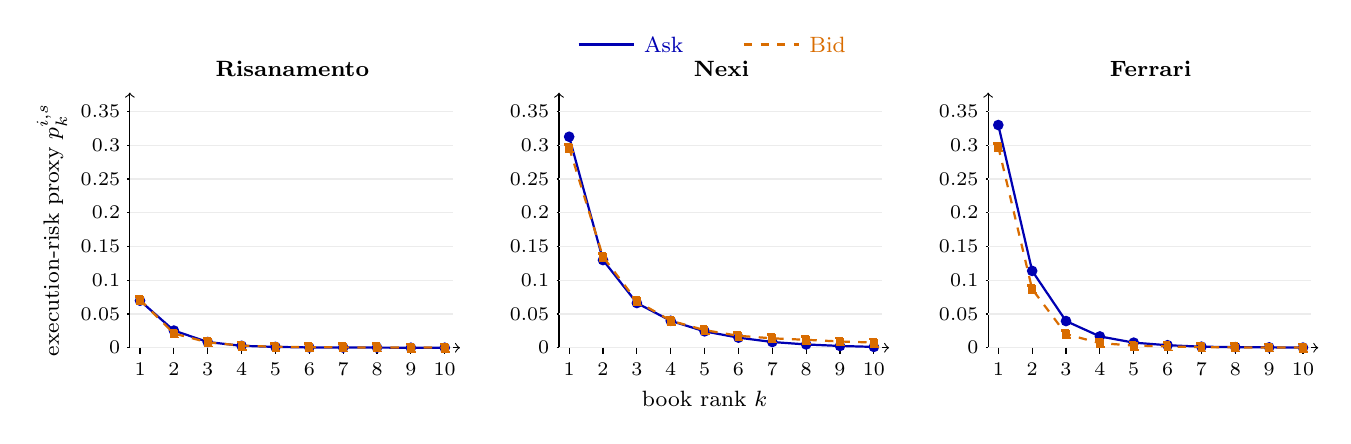
\begin{tikzpicture}
\begin{scope}[xshift=0.00cm]
\begin{scope}[x=0.43cm,y=8.57142857cm]
  \draw[->] (0.7,0) -- (10.45,0);
  \draw[->] (0.7,0) -- (0.7,0.378);
  \draw[gray!15] (0.7,0) -- (10.25,0);
  \draw (0.63,0) -- (0.7,0) node[left,font=\scriptsize] {0};
  \draw[gray!15] (0.7,0.05) -- (10.25,0.05);
  \draw (0.63,0.05) -- (0.7,0.05) node[left,font=\scriptsize] {0.05};
  \draw[gray!15] (0.7,0.1) -- (10.25,0.1);
  \draw (0.63,0.1) -- (0.7,0.1) node[left,font=\scriptsize] {0.1};
  \draw[gray!15] (0.7,0.15) -- (10.25,0.15);
  \draw (0.63,0.15) -- (0.7,0.15) node[left,font=\scriptsize] {0.15};
  \draw[gray!15] (0.7,0.2) -- (10.25,0.2);
  \draw (0.63,0.2) -- (0.7,0.2) node[left,font=\scriptsize] {0.2};
  \draw[gray!15] (0.7,0.25) -- (10.25,0.25);
  \draw (0.63,0.25) -- (0.7,0.25) node[left,font=\scriptsize] {0.25};
  \draw[gray!15] (0.7,0.3) -- (10.25,0.3);
  \draw (0.63,0.3) -- (0.7,0.3) node[left,font=\scriptsize] {0.3};
  \draw[gray!15] (0.7,0.35) -- (10.25,0.35);
  \draw (0.63,0.35) -- (0.7,0.35) node[left,font=\scriptsize] {0.35};
  \draw (1,0) -- (1,-0.025 * 0.35) node[below,font=\scriptsize] {1};
  \draw (2,0) -- (2,-0.025 * 0.35) node[below,font=\scriptsize] {2};
  \draw (3,0) -- (3,-0.025 * 0.35) node[below,font=\scriptsize] {3};
  \draw (4,0) -- (4,-0.025 * 0.35) node[below,font=\scriptsize] {4};
  \draw (5,0) -- (5,-0.025 * 0.35) node[below,font=\scriptsize] {5};
  \draw (6,0) -- (6,-0.025 * 0.35) node[below,font=\scriptsize] {6};
  \draw (7,0) -- (7,-0.025 * 0.35) node[below,font=\scriptsize] {7};
  \draw (8,0) -- (8,-0.025 * 0.35) node[below,font=\scriptsize] {8};
  \draw (9,0) -- (9,-0.025 * 0.35) node[below,font=\scriptsize] {9};
  \draw (10,0) -- (10,-0.025 * 0.35) node[below,font=\scriptsize] {10};
  \node[rotate=90,font=\footnotesize] at (-1.6,0.175) {execution-risk proxy $p_k^{i,s}$};
  \node[font=\footnotesize\bfseries] at (5.5,0.413) {Risanamento};
  \draw[blue!70!black, thick, mark=*, mark size=1.5pt] plot coordinates {(1,0.06972349940165018) (2,0.02545533573561784) (3,0.008478028770510227) (4,0.0028297304716921367) (5,0.0012412635498727) (6,0.0004097636793952453) (7,0.0002830315509421413) (8,0.00021971635327554557) (9,0.0) (10,0.0)};
  % RISANAMENTO ask hit_probability raw: 1:0.06972349940165018, 2:0.02545533573561784, 3:0.0084780287705102271, 4:0.0028297304716921367, 5:0.0012412635498726999, 6:0.0004097636793952453, 7:0.0002830315509421413, 8:0.00021971635327554557, 9:0, 10:0
  \draw[orange!85!black, thick, dashed, mark=square*, mark size=1.4pt] plot coordinates {(1,0.07096878130100093) (2,0.021101548570064722) (3,0.007994257645916313) (4,0.0031324298201674864) (5,0.0014088794806261372) (6,0.0008309423027754893) (7,0.0005630550368480321) (8,0.0003863103073313112) (9,0.00020106276030446647) (10,0.00018748873264827834)};
  % RISANAMENTO bid hit_probability raw: 1:0.070968781301000927, 2:0.021101548570064722, 3:0.0079942576459163129, 4:0.0031324298201674864, 5:0.0014088794806261372, 6:0.00083094230277548935, 7:0.00056305503684803214, 8:0.00038631030733131118, 9:0.00020106276030446647, 10:0.00018748873264827834
\end{scope}
\end{scope}
\begin{scope}[xshift=5.45cm]
\begin{scope}[x=0.43cm,y=8.57142857cm]
  \draw[->] (0.7,0) -- (10.45,0);
  \draw[->] (0.7,0) -- (0.7,0.378);
  \draw[gray!15] (0.7,0) -- (10.25,0);
  \draw (0.63,0) -- (0.7,0) node[left,font=\scriptsize] {0};
  \draw[gray!15] (0.7,0.05) -- (10.25,0.05);
  \draw (0.63,0.05) -- (0.7,0.05) node[left,font=\scriptsize] {0.05};
  \draw[gray!15] (0.7,0.1) -- (10.25,0.1);
  \draw (0.63,0.1) -- (0.7,0.1) node[left,font=\scriptsize] {0.1};
  \draw[gray!15] (0.7,0.15) -- (10.25,0.15);
  \draw (0.63,0.15) -- (0.7,0.15) node[left,font=\scriptsize] {0.15};
  \draw[gray!15] (0.7,0.2) -- (10.25,0.2);
  \draw (0.63,0.2) -- (0.7,0.2) node[left,font=\scriptsize] {0.2};
  \draw[gray!15] (0.7,0.25) -- (10.25,0.25);
  \draw (0.63,0.25) -- (0.7,0.25) node[left,font=\scriptsize] {0.25};
  \draw[gray!15] (0.7,0.3) -- (10.25,0.3);
  \draw (0.63,0.3) -- (0.7,0.3) node[left,font=\scriptsize] {0.3};
  \draw[gray!15] (0.7,0.35) -- (10.25,0.35);
  \draw (0.63,0.35) -- (0.7,0.35) node[left,font=\scriptsize] {0.35};
  \draw (1,0) -- (1,-0.025 * 0.35) node[below,font=\scriptsize] {1};
  \draw (2,0) -- (2,-0.025 * 0.35) node[below,font=\scriptsize] {2};
  \draw (3,0) -- (3,-0.025 * 0.35) node[below,font=\scriptsize] {3};
  \draw (4,0) -- (4,-0.025 * 0.35) node[below,font=\scriptsize] {4};
  \draw (5,0) -- (5,-0.025 * 0.35) node[below,font=\scriptsize] {5};
  \draw (6,0) -- (6,-0.025 * 0.35) node[below,font=\scriptsize] {6};
  \draw (7,0) -- (7,-0.025 * 0.35) node[below,font=\scriptsize] {7};
  \draw (8,0) -- (8,-0.025 * 0.35) node[below,font=\scriptsize] {8};
  \draw (9,0) -- (9,-0.025 * 0.35) node[below,font=\scriptsize] {9};
  \draw (10,0) -- (10,-0.025 * 0.35) node[below,font=\scriptsize] {10};
  \node[font=\footnotesize\bfseries] at (5.5,0.413) {Nexi};
  \draw[blue!70!black, thick, mark=*, mark size=1.5pt] plot coordinates {(1,0.31260453781443537) (2,0.12984782045855234) (3,0.06622282497020507) (4,0.03985550427610355) (5,0.024238887427669647) (6,0.014926477236300272) (7,0.008478372547005035) (8,0.004874179588448276) (9,0.002609710589260322) (10,0.0012329392037678621)};
  % NEXI ask hit_probability raw: 1:0.31260453781443537, 2:0.12984782045855234, 3:0.066222824970205069, 4:0.03985550427610355, 5:0.024238887427669647, 6:0.014926477236300272, 7:0.0084783725470050347, 8:0.0048741795884482764, 9:0.0026097105892603219, 10:0.0012329392037678621
  \draw[orange!85!black, thick, dashed, mark=square*, mark size=1.4pt] plot coordinates {(1,0.2962844238411685) (2,0.13459420361328928) (3,0.06890514548742396) (4,0.040104226602442915) (5,0.02609796394782051) (6,0.017697805652940525) (7,0.013941406635320423) (8,0.011730229384758923) (9,0.009260324871761146) (10,0.007653260445138618)};
  % NEXI bid hit_probability raw: 1:0.29628442384116849, 2:0.13459420361328928, 3:0.068905145487423963, 4:0.040104226602442915, 5:0.026097963947820511, 6:0.017697805652940525, 7:0.013941406635320423, 8:0.011730229384758923, 9:0.0092603248717611462, 10:0.0076532604451386181
\end{scope}
\end{scope}
\begin{scope}[xshift=10.90cm]
\begin{scope}[x=0.43cm,y=8.57142857cm]
  \draw[->] (0.7,0) -- (10.45,0);
  \draw[->] (0.7,0) -- (0.7,0.378);
  \draw[gray!15] (0.7,0) -- (10.25,0);
  \draw (0.63,0) -- (0.7,0) node[left,font=\scriptsize] {0};
  \draw[gray!15] (0.7,0.05) -- (10.25,0.05);
  \draw (0.63,0.05) -- (0.7,0.05) node[left,font=\scriptsize] {0.05};
  \draw[gray!15] (0.7,0.1) -- (10.25,0.1);
  \draw (0.63,0.1) -- (0.7,0.1) node[left,font=\scriptsize] {0.1};
  \draw[gray!15] (0.7,0.15) -- (10.25,0.15);
  \draw (0.63,0.15) -- (0.7,0.15) node[left,font=\scriptsize] {0.15};
  \draw[gray!15] (0.7,0.2) -- (10.25,0.2);
  \draw (0.63,0.2) -- (0.7,0.2) node[left,font=\scriptsize] {0.2};
  \draw[gray!15] (0.7,0.25) -- (10.25,0.25);
  \draw (0.63,0.25) -- (0.7,0.25) node[left,font=\scriptsize] {0.25};
  \draw[gray!15] (0.7,0.3) -- (10.25,0.3);
  \draw (0.63,0.3) -- (0.7,0.3) node[left,font=\scriptsize] {0.3};
  \draw[gray!15] (0.7,0.35) -- (10.25,0.35);
  \draw (0.63,0.35) -- (0.7,0.35) node[left,font=\scriptsize] {0.35};
  \draw (1,0) -- (1,-0.025 * 0.35) node[below,font=\scriptsize] {1};
  \draw (2,0) -- (2,-0.025 * 0.35) node[below,font=\scriptsize] {2};
  \draw (3,0) -- (3,-0.025 * 0.35) node[below,font=\scriptsize] {3};
  \draw (4,0) -- (4,-0.025 * 0.35) node[below,font=\scriptsize] {4};
  \draw (5,0) -- (5,-0.025 * 0.35) node[below,font=\scriptsize] {5};
  \draw (6,0) -- (6,-0.025 * 0.35) node[below,font=\scriptsize] {6};
  \draw (7,0) -- (7,-0.025 * 0.35) node[below,font=\scriptsize] {7};
  \draw (8,0) -- (8,-0.025 * 0.35) node[below,font=\scriptsize] {8};
  \draw (9,0) -- (9,-0.025 * 0.35) node[below,font=\scriptsize] {9};
  \draw (10,0) -- (10,-0.025 * 0.35) node[below,font=\scriptsize] {10};
  \node[font=\footnotesize\bfseries] at (5.5,0.413) {Ferrari};
  \draw[blue!70!black, thick, mark=*, mark size=1.5pt] plot coordinates {(1,0.3299702364891511) (2,0.1138451000944385) (3,0.039512737809105136) (4,0.016772763406691257) (5,0.007550976354941552) (6,0.0037028504060889473) (7,0.0015255640954857832) (8,0.0008800569546293279) (9,0.0005811708933011752) (10,0.00019095892515032825)};
  % FERRARI ask hit_probability raw: 1:0.32997023648915108, 2:0.1138451000944385, 3:0.039512737809105136, 4:0.016772763406691257, 5:0.0075509763549415519, 6:0.0037028504060889473, 7:0.0015255640954857832, 8:0.00088005695462932789, 9:0.00058117089330117521, 10:0.00019095892515032825
  \draw[orange!85!black, thick, dashed, mark=square*, mark size=1.4pt] plot coordinates {(1,0.29774219794269774) (2,0.08683487342980731) (3,0.0201937386748806) (4,0.006785226513236277) (5,0.003250439515049369) (6,0.0018722238366059196) (7,0.0007970509116269802) (8,0.0005189144310103264) (9,0.0003238052933862769) (10,0.00017228173668293312)};
  % FERRARI bid hit_probability raw: 1:0.29774219794269774, 2:0.086834873429807308, 3:0.020193738674880599, 4:0.0067852265132362774, 5:0.003250439515049369, 6:0.0018722238366059196, 7:0.00079705091162698017, 8:0.00051891443101032637, 9:0.0003238052933862769, 10:0.00017228173668293312
\end{scope}
\end{scope}
\node[font=\footnotesize] at (7.6,-0.65) {book rank $k$};
\draw[blue!70!black,thick,mark=*,mark size=1.5pt] (6.0,3.85) -- (6.7,3.85) node[right,font=\footnotesize] {Ask};
\draw[orange!85!black,thick,dashed,mark=square*,mark size=1.4pt] (8.1,3.85) -- (8.8,3.85) node[right,font=\footnotesize] {Bid};
\end{tikzpicture}%
}
\caption{Side-specific empirical execution-risk proxy by book rank. The plotted quantity is the stored $h$-second reach probability $p_k^{i,s}$ (\texttt{hit\_probability}) from the full-sample top-$10$, $h=10$-second calibration. The empirical kernel uses its protection complement $\rho_k^{i,s}=1-p_k^{i,s}$.}
\label{fig:empirical_topn_execution_risk_profiles}
\end{figure}
